\documentclass[output=paper]{langscibook}
\ChapterDOI{10.5281/zenodo.4545047}

\author{Hanna Risku\affiliation{University of Vienna} and Barbara Meinx\affiliation{Oesterreichische Nationalbank}}
\title{Emotion and the social embeddedness of translation in the workplace}
\abstract{This paper examines the emotional aspects of the translation process while taking into account the social embeddedness of translators in their working environments. It explores how it feels to be a translator, looks at what makes translators thrive or despair and examines how they cope emotionally with their work circumstances. The empirical setting for this qualitative workplace study is the translation department of an Austrian public sector institution, where authentic work situations were investigated using ethnographic research methods, i.e., participatory observation and semi-structured expert interviews. The results indicate that the translators in this department experience a wide variety of emotions ranging from satisfaction, pride, relief and enjoyment to stress, disappointment and frustration. These are inextricably linked with the networks, actors and environments involved in the translation processes and occasionally lead to the use of coping strategies.}


\begin{document}
\maketitle

\section{Introduction} 
Translation process research has increasingly begun to emphasise the role of affective and attitudinal factors in translation \citep{Laukkanen1996}. Psychological aspects like translator personality \citep{Hubscher-Davidson2009} and ergonomic aspects like translator well-being \citep{Ehrensberger-Dow2018} are attracting increasing attention as explanatory factors of translation activities and processes. At the same time, the role of emotions in translation has become a legitimate object in translation process research.

This paper focuses on how it feels to be a translator, what makes translators thrive or despair and how they deal emotionally with their work circumstances. Accordingly, it examines both the emotional aspects of the translation process and the social embeddedness of translators in their real working environments, concentrating thereby on three research questions: (1) Which emotions do translators experience during a translation process? (2) Which factors trigger emotions in translators and how do these relate to the social setting in which they work? (3) Do translators apply strategies to deal with emotions?

Before describing and discussing our research results, we will first provide an outline of prior empirical research on emotional aspects of translation as well as a brief discussion of the topic of emotions from the psychological, cognitive and situated perspectives.

\section{Emotions as an object of translation process research}
Emotion variables have already been mentioned in various studies of the translation process (e.g., \citealp{Kußmaul1991, Tirkkonen-Condit1996, Jääskeläinen1996, Davou2007, RojoLópez2014, RojoLópez2016, Hubscher-Davidson2009, Hubscher-Davidson2013, Lehr2014}). They have been described as an area of relevance to translation process research in which a number of aspects have yet to be explored.

Kußmaul provides a detailed description of the influence of positive emotions on the translation process. In a 1991 study examining the processes involved in the development of creative solutions to translation problems, he asked two translators to work as a team to translate a text from English into German and to explain and discuss their methods with each other while they worked. The resulting dialogue protocols led Kußmaul to conclude that the creative solutions which emerge during the translation process are linked to situations in which the translators experience positive emotions. This finding is reiterated in a 2007 study by Davou.

\citet{RojoLópez2014} show that negative emotions can have adverse effects on the translation process. They used a reaction time experiment to examine the influence of words and expressions which contradict the translator’s own ideological stance. The results corroborate their assumption that words and expressions that are incompatible with a translator’s ideology have an adverse effect on the decision process and lead to more time being required to find an adequate translation solution. By contrast, words and expressions that are compatible with the translator's ideology facilitate the decision process, allowing a suitable translation to be found more quickly.

\citeauthor{Lehr2014}'s (\citeyear{Lehr2014}) results indicate that the emotions triggered in translators through feedback on completed translations influence subsequent translation processes in different ways depending on their valence (positive or negative). Feedback that prompts positive emotions enhances idiomatic expression and stylistic appropriateness in subsequent translations, while feedback that prompts negative emotions enhances coherence and correctness of terminology.

\citeauthor{RojoLópez2016} repeated Lehr’s study in 2016 and reached similar conclusions. In addition to replicating her methodology, they used Block \& Kremen’s ego-resiliency scale to explore the influence of personality traits on the translation process. Their results show that positive and negative emotions triggered by feedback on performance lead to different processing styles, increasing either creativity or accuracy in translation. They also suggest that personality traits play a role~-- albeit not a statistically significant one -- in guiding translational behaviour.

\section{Emotions from the psychological, cognitive and situated perspectives}
From a psychological perspective, emotional and affective phenomena are positioned on a spectrum ranging from acute, physiological changes (e.g. intense fear) through to more stable personality traits (e.g. irritability) \citep[40]{Davou2007}. According to \citet[322]{Ekkekakis2012}, \textit{emotions} “are elicited \textit{by} something, are reactions \textit{to} something, and are generally \textit{about} something". Conversely, \textit{core affects} (such as pleasure, tiredness or tension) are consciously accessible states that are experienced on an ongoing basis, albeit with varying levels of intensity. Unlike emotions, they do not relate to specific situations (including people, events or things, whether past, present, future, real or imagined). Similarly, it is not always easy to identify the causes and stimuli of \textit{moods}, which differ from emotions in that they typically last longer and tend to be diffuse and global rather than specific \citep[322]{Ekkekakis2012}.

Along with the recent reorientation in cognitive science towards a more situated, embodied and distributed understanding, emotions have entered the field as central elements of cognition. It is now increasingly acknowledged that emotion and cognition are indeed inseparable. Emotions play a critical role in all -- also high-level -- cognition and decision-making \citep{Damasio1994, Damasio1999}: they drive cognition, make it meaningful and steer our attention and motivations. From this point of view, emotions are allocated a primary role in cognition, and it is emotion that “enslaves” the brain and moves the body. Nevertheless, emotions have not undergone such a revolutionary redefinition as cognitive phenomena in cognitive translation studies.

Embodied cognition approaches underline the notion that cognition consists of or is enacted through interaction with social and physical environments. According to \citet[67]{Stephan2014}, this also applies to emotions, since neither our modes of thinking nor the way we feel occur in isolation. This calls for an approach which takes into account that cognitive and emotional processes are “possibly (1) linked to our physical state (i.e. are ‘embodied’), and (2) dependent on our environment (i.e. are ‘embedded’), and thus might therefore (3) go beyond the limits of our body (i.e. be ‘extended’), and (4) only develop in the interaction with our environment (i.e. be ‘enacted’)” \citep[285; translated by the authors]{Wilutzky2011}.

\citet[438]{Griffiths2009} support such an approach and demonstrate that the adoption of a situated perspective goes hand in hand with a reorientation in research into emotions:

\begin{quote}\sloppy
    By shifting theoretical focus from the intrapsychic to the interpersonal, from the unbidden to the strategic, from the short-lived to the long-lived, from the context-independent to the context-dependent, from the static to the dynamic, the situated perspective points the attention of the research community to aspects of emotions that have been unduly neglected and that may hold the key to understanding the nature and function of a large class of emotions. \citep[448f]{Griffiths2009}
\end{quote}

\noindent
They thus reject the cognitivist understanding of emotions as merely evaluative judgments of internal cognitive representations. This definition might not make sense if cognition or intelligence is not about internally representing the environment and manipulating these representations but rather about (inter)acting in the environment. They also maintain that the situated view of emotions identifies them as “acts of relationship reconfiguration” in a social context and as “forms of skillful engagement with the world […] scaffolded by […] and dynamically coupled to an environment” \citep[438]{Griffiths2009}.

This “transactional” and situated view of emotions as temporal processes of continuous exchange with the (social and material) environment thus constitutes an “affective parallel” to the situated view of cognition \citep[438]{Griffiths2009}. Situated approaches therefore view emotions as material and social interactions that are best studied from a process and network perspective.

\section{Research design and case study setting}
This is precisely the perspective adopted for our study, which aims to illustrate the relevance of the social environment and processes for the emotions triggered in translators at the workplace. To achieve this, we examined authentic translation processes using qualitative ethnographic methods (participatory observation and semi-structured expert interviews). While participatory observation in the translation workplace provides insights into the emotional content of translation processes and translators’ interactions with their environment, semi-structured interviews serve to reconstruct the translation processes in their entirety from the (emotional) perspective of the translators. The empirical setting for our case study is the translation department (working languages: German and English) of an Austrian public sector institution, where we conducted observation sessions and seven interviews over a period of 17 working days. Five of the seven interviews were conducted with the department’s inhouse translators (T1--T5), one with a retired colleague (T6) who now works for the department on a freelance basis and one with the head of the department.

Participatory observation is a standard field research method in which the researchers do not passively observe the object of study but instead actively participate in the situation in which it is embedded. The researchers thus interact directly with those being studied and collect data by participating in their everyday situation \citep[80]{Mayring2002}. In our participatory observation of the aforementioned translation department, our prerogative was therefore to be open to all manner of different aspects and to take copious field notes that recorded these as precisely as possible. Since this faced us with the problem that not all phenomena in a situation can always be noted down immediately, we expanded our field notes during breaks in and directly after the individual observation periods. Moreover, to enable the researchers to reconstruct the broader context and experience behind the observed actions, participatory observation -- as was the case in our study -- frequently relies on questions being posed during the observation sessions (\citealp[82]{Mayring2002}; \citealp[295]{Flick2002}).

Expert interviews are generally conducted as so-called guided interviews. Accordingly, they are based on a list of open questions (the interview guideline) that is prepared in advance; they are also defined by the specific choice and status of the interviewees (the experts) (\citealp[111]{Gläser2009}; \citealp[559]{Helfferich2014}). When preparing the guideline, researchers are recommended to keep it as open as possible and as structured as necessary \citep[566]{Helfferich2014}, an approach we likewise adopted when preparing the interview guideline for our own interviews. Our interview guideline (see Appendix~\ref{sec:10:appendix}) thus incorporated open requests to talk about the spectrum of activities involved in the translators' own work and any frequently occurring processes therein. It also included questions on the social network and any artefacts (tools) required to fulfil the translators' tasks. Finally, the topic of emotions experienced during translation processes was explicitly raised. We thereby chose not to use predefined lists of emotions -- a common approach in such interviews \citep[712]{Scherer2005} -- since we wanted our experts to talk freely and in their own words about emotional events. We also felt that their work setting could trigger complex emotions that would not necessarily fit into predefined emotion categories. Furthermore, since some of our questions were already covered in the topics raised by the interviewees, we did not always need to ask all the questions in our guideline or keep to the predefined order of questions. In fact, we felt it was more important to give the interviewees space to say what they wanted to say and address the topics that were important to them -- regardless of the order in which they were raised.

Both the audio recordings of the interviews and the field notes taken during the observations were then transcribed using an adapted version of the conventions described in \citet{Selting2011}. This was followed by a software-assisted (MAXQDA) qualitative analysis of the interview and observation protocols in line with the qualitative content analysis method proposed by \citet{Gläser2009}. This method helps to extract the relevant information, i.e., it separates it from the original empirical material by applying a set of categories that can be developed deductively from prior theory, inductively by a data-driven procedure, or -- as in our case -- using a combination of both these strategies \citep[21f]{Gläser2013}.

To extract the relevant information from our data, we used six very general deductive categories derived from the \textit{dynamic network model of translatorial cognition and action} by \citet{Risku2013}, namely “cognition", “action", “social network", “artefacts", “environments" and “time". Within these categories, we constructed a number of emotional subcategories that emerged inductively from the data we had gathered and ranged from enjoyment and satisfaction to frustration and disappointment (see Table~\ref{tab:Nodes}). These emotions were either clearly defined as such by the translators or inferred from the statements recorded in the interviews as well as the comments, actions, gestures and facial expressions noted during the observation sessions. In doing so, we used the aforementioned situated view of emotions as the relational and interactive qualities of what is said and done as a basis for identifying emotions. We then checked the extracted and categorised raw data segments for redundancies and contradictions and sorted them by aspects relevant to our analysis. This structured information base was then used to analyse and interpret the relevant data in line with our research questions \citep[202f]{Gläser2009}.

\begin{table}
        \caption{Emotions related to the nodes in the social network}
        \label{tab:Nodes}
        \begin{tabularx}{.8\textwidth}{lX}
            \lsptoprule
            Nodes & Emotions\\\midrule
            Translation team                & \begin{tabular}[c]{@{}l@{}}Enjoyment\\Ownership\\Satisfaction\end{tabular}\\\midrule
            Source text authors (= clients) & \begin{tabular}[c]{@{}l@{}}Anger\\Aversion\\Caution/wariness\\Enjoyment\\Impotence\\Reluctance\\Stress~\end{tabular}\\\midrule
            Management             & \begin{tabular}[c]{@{}l@{}}Dissatisfaction\\Frustration\\Impotence\\Interest\\Pride ~\end{tabular}\\  \midrule
            External translators   & \begin{tabular}[c]{@{}l@{}}Enjoyment\\Relief\end{tabular} \\\midrule
            (Non-existent) readers & Disappointment \\
            \lspbottomrule
        \end{tabularx}
    \end{table}

\section{Research results}\label{sec:10:results}
The results obtained from our interviews and observations indicate that the translators working in this public sector institution  are members of a complex social network. As Figure~\ref{fig:socialnetwork} shows, the translation department (indicated in dark blue) is part of a larger department (light blue), which, in turn, is part of the institution-wide social network (grey).

\begin{figure}
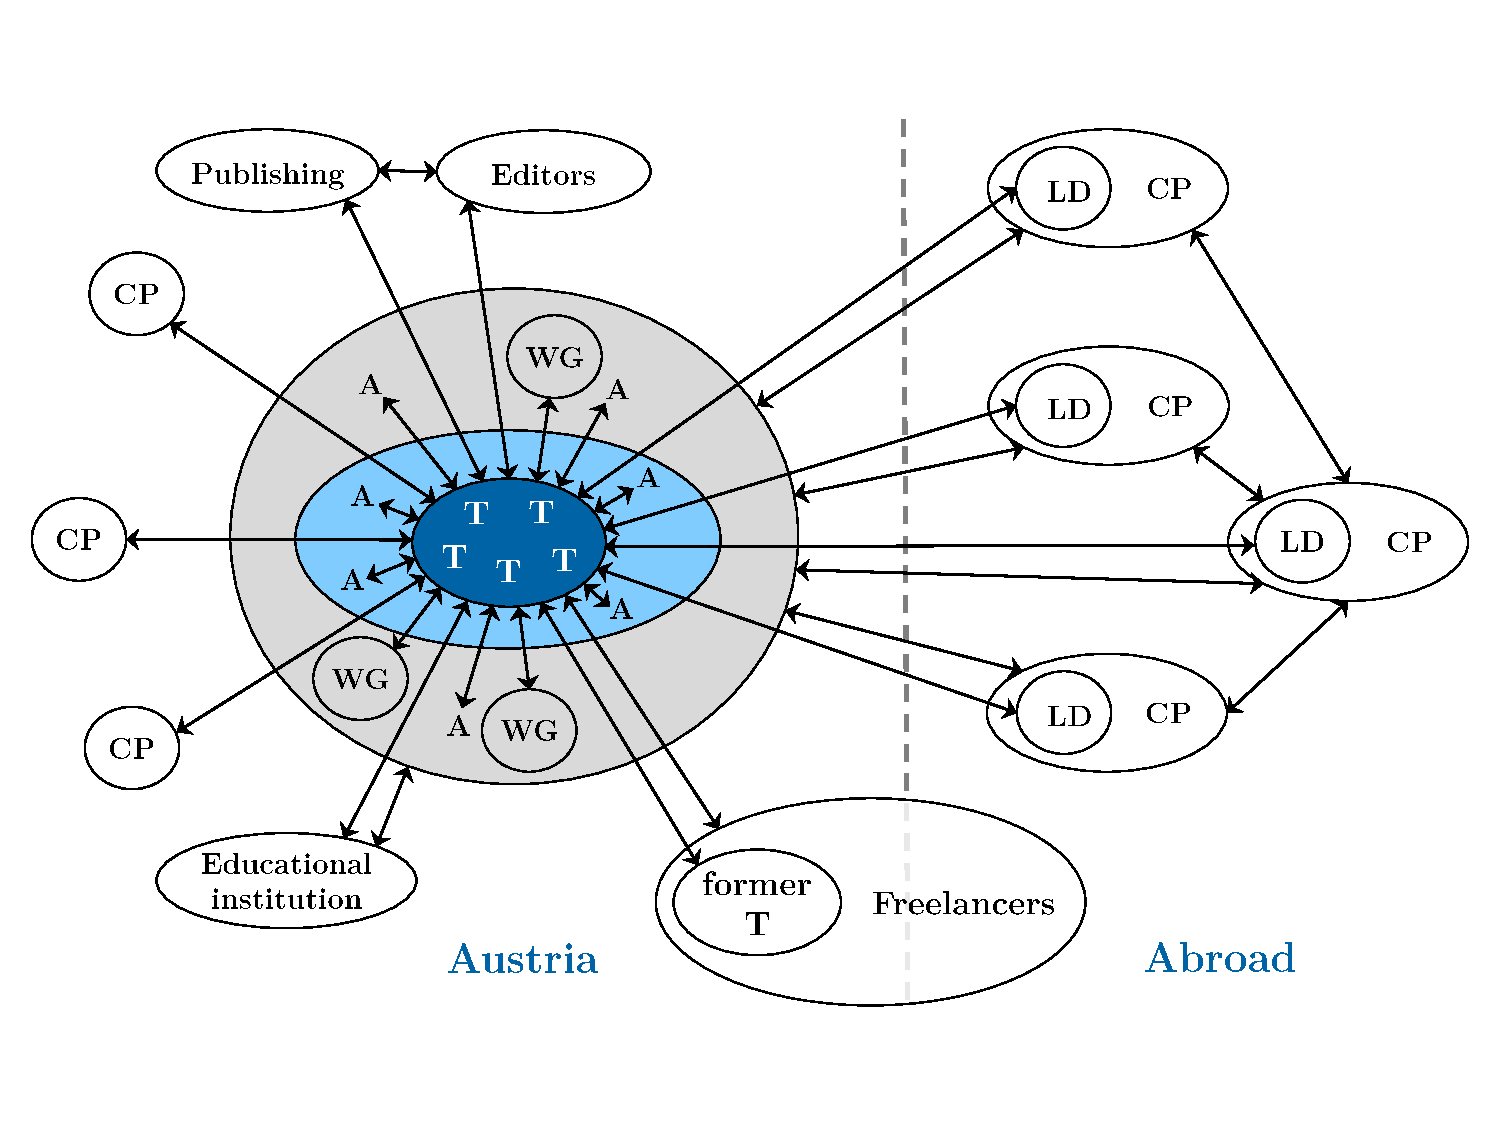
\includegraphics[width=1\textwidth]{figures/SocialNetwork.pdf}
\caption{The translation department's social network\label{fig:socialnetwork}}
\small
\begin{tabular}{r@{: }l r@{: }l}
CP& Cooperation partner & WG& Working group\\
LD& Language department & A& Author 
\end{tabular}
\end{figure}

As voiced in the interviews and noted in the observations, the translators experience a multitude of different emotions in relation to their social embeddedness in this network. These range from satisfaction, pride, relief and enjoyment to interest, caution and ownership (the feeling of having to stand up for themselves and take sides). They also include disappointment, aversion or reluctance as well as stress, a sense of impotence and even frustration and anger.

The emotions detected in our analysis relate to the following nodes in the social network: the translation team, source text authors (as clients of the translation department), management, external translators and readers (see Table~\ref{tab:Nodes}). Since discussing all the emotions detected would exceed the scope of this paper, we have restricted ourselves to one or two examples for each node.

\subsection{Translation team: Satisfaction}

The translators appear to be largely satisfied with the underlying structures in their team. For example, they hold an annual meeting to decide who will assume responsibility for which publications in the coming year and thus for the corresponding proofreading, translation and administrative tasks (Interview T3).

A regular meeting is also held every two weeks to enable the translators to keep each other updated. When talking about this meeting, T6 notes: “We were a bit sceptical and worried at the beginning because it’s very structured, yet now we really wouldn’t want to be without it. It’s a very important way for us to share information” (Interview T6).

T1 points out that inconsistencies in the past had necessitated this sharing of tasks, and that they had developed this approach themselves in a professional supervision project. She also explains that the department had begun expanding rapidly around two years after she joined and that “there had to be some reallocation of responsibilities and rotations etc. so that everyone was satisfied with the way the work was shared. […] [The supervision project] clearly helped us a lot because all our structures are still based on what we agreed back then” (Interview~T1).

\subsection{Source text authors: Stress}

Resources within the translation department are extremely limited. The team had previously consisted of six translators and had been able to handle its workload relatively easily, even at peak times. It has since been reduced to 4.5 full-time equivalents, which according to T5 “is okay but not always easy, especially when someone’s away, e.g. ill, on a business trip or on holiday. […] We sometimes have ridiculous amounts of holiday left over that never get used. It’s just really busy” (Interview T5).

This heavy workload could also be clearly observed, especially when the translators had to meet very tight deadlines. Yet they appear to take it in their stride: “Why do [the clients] have to get so stressed out about it, like it’s the first time we’ve ever had something come in at the last minute?” (Observation T2).\linebreak Nonetheless, the translators' reactions to such tight deadlines do differ. According to T4, some of them take a “we’ll manage it somehow” attitude, while others say: “They must be joking. If [the client] needs a long text like that […] we’ll need more time” (Interview T4).

Despite the differences of opinion regarding manageable workload, the translators do their best to handle such (large) texts within the team. “We split texts up: I do a couple of pages, [T5] does a couple of pages, and someone else does the quality assurance” (Interview T3). The department also asks its clients to let them know in advance about large texts so it can plan ahead and assign tasks accordingly (Interview T3). “But sometimes you do have to tell the client if it’s not possible and try to educate them” (Interview T5).

\subsection{Management: Frustration and impotence}

T6, whose position was not filled after she retired, laments the staff cutbacks in the department: “Savings start lower down the ladder. […] The [authors] are sacred, and [the translation department] is a support function. So it’s an easy place to start cutting costs whilst still profiting from the fact that [the translation department] raises the quality of the work” (Interview T6).

T5 expresses frustration at the lack of appreciation for the department that is encountered in the organisation as a whole. Some managers do not even see the need for a translation department “because everyone can speak English anyway, and we can just do it ourselves” (Interview T5). This frustration is shared by T1 and T4, who explain that the department’s work is frequently taken for granted and that it only receives any attention if something has not gone well (Interview~T4). “It’s the typical service problem. If you get any feedback at all, then only when someone isn’t happy with something” (Interview T1).

The translators also feel powerless in the face of economic or policy decisions made within the organisation such as the recent decision that authors should draft their texts in English and the translators should simply proofread them -- a decision which has since been implemented for the majority of publications. “We often don’t understand the cost-cutting policy. […] And then they think it’s a really good idea that -- because we’ve got one less person -- we should outsource texts or just not translate them” (Interview T2).

Yet T2 has also given great thought to how she can be actively involved in this changing work environment, provide added value and continue to enjoy her work. She now supports authors in drafting texts in English by organising writing courses and compiling style guides and lists of useful phrases (Observation~T2).

\subsection{External translators: Relief and enjoyment}

The members of the translation department express relief in the fact that they can draw on a relatively large pool of good external translators and proofreaders with whom they have worked for many years (Interview T1). These include two of their own former colleagues, whose familiarity with the organisation and internal know-how make them highly valuable resources (Observation T4).

Further assistance is obtained through cross-institutional collaboration with other translation departments. In exchange programmes lasting several weeks, colleagues from other institutions have the opportunity to “join” the translation department and work alongside the inhouse translators. According to T2, having an additional translator support them for a couple of weeks is very helpful (Observation T2).

T3 enjoys the reciprocal nature of this programme, which has already given her the opportunity to work on another organisation’s annual report on four occasions. She describes this as “a great way to work” and a chance to “learn so much” (Interview T3). She is likewise pleased that her initial concerns about joining the organisation have proved unfounded:

\begin{quote}
    When I accepted this job, I had the horrifying vision that I’d be sitting in front of a computer all day long with no contact to other people. […] I'm so glad that this nightmarish thought does not reflect reality. We actually have a lot of contact with the authors, the people in our own team or translators in other institutions. (Interview T3)
\end{quote}

\subsection{Readers: Disappointment}

The emotion of disappointment refers here to the feeling that you experience when you realise that something is not what you hoped it would be. Perhaps due to her quality awareness for proofreading and translation, T5 often has the feeling that she is to some extent working for “nothing” (Interview T5). While the translation department puts great effort into delivering texts that are useful and readily understandable for the target reader, she notes that:

\begin{quote}
    […] with some types of publication, you think from the outset that no one will ever read this. That often makes it difficult from the sense perspective, so you sometimes just have to concentrate more on your pay slip and think, ``okay, I’ve finished that now, it’s part of my work, I get paid for it, and it pays the bills''. I find that quite hard because I love creating a beautiful text but when you know full well that it will probably only be read by about three people, you find yourself wondering whether it’s a meaningful use of your time. But it’s always a very mixed bag. (Interview T5)
\end{quote}

\noindent
On rare occasions, T4 also finds herself wondering whether she couldn’t have chosen a more meaningful job (Interview T4). “But that usually passes again”, she adds, “then a nice piece of work comes along, and you think, ‘oh yes, people will want to read this’ or that you have made a meaningful contribution to something” (Interview T4).

\section{Discussion}
While the qualitative study described in this article assigns high priority to the ecological validity of its design, it is also a case study based on a small number of participants, and its findings cannot thus be generalised. Nonetheless, since articles on the topic of emotions are still thin on the ground in translation studies, and few empirical studies as yet address the social embeddedness of emotions in the translation workplace, we felt that a qualitative approach was best suited to obtaining an initial insight into the situative, emotional processes related to social aspects in the translation process.

As can be seen from the examples presented in Section~\ref{sec:10:results}, the translators in our study experience a wide range of emotions in relation to their social network in the course of translation processes. While the emotions triggered by working in their own team and with external translators are largely positive, those relating to the institution-wide social network are somewhat mixed.

Our study also provides examples of how translators apply strategies to deal with emotions. In this regard, emotions can be seen as elements of strategies to meaningfully interact with the environment and reconfigure relationships. A review of the negatively valenced emotions triggered by the social network indicates that these did not result in acquiescence but rather in the translators becoming proactive and seeking solutions to problems. Strategies to manage stressful situations within the team have likewise proved effective despite the differences of opinion regarding manageable workload. Strategies have also emerged to deal with developments beyond the translators’ control, i.e., the growing importance of English as a lingua franca and the corresponding increase in proofreading and editing tasks due to the switch to mostly English-language publications in the organisation.

\section{Conclusions}
From an emotional embeddedness perspective, our results provide examples of how the emotions experienced by translators can be studied as “enacted in the interaction with [their] environment” \citep[285]{Wilutzky2011} and as “forms of skillful engagement with the world […] scaffolded by […] and dynamically coupled to an environment” \citep[438]{Griffiths2009}.

Our study also indicates that qualitative ethnographic methods like participatory observation and semi-structured expert interviews can be included in the methodological toolkit of translation scholars studying the emotional aspects of translation, alongside other tools like focus groups, translators’ own narrations in diaries or ``fictive love and break-up letters'' \citep{Ruokonen2017} and controlled experiments using, for example, verbal reports or psychophysiological measures. Specifically, workplace research using participatory observation and semi-structured expert interviews provides a way to take account of the translators’ social environments and processes. Accordingly, it could be used in future studies to explore how emotions are triggered in translators embedded in different social contexts, thus helping to fill the gaps in our knowledge when it comes to translation and emotions, especially in the situated context.


\appendixsection{Interview guideline}: \label{sec:10:appendix}

\appendixsubsection*{Initial topics} career history, length of time in translation department, responsibilities


\appendixsubsection{Processes}
\begin{itemize}
\itemsep0em
    \item Ask about the interviewee’s own tasks: How would you describe the work you do? (e.g. translation, reviewing, copyediting, etc.) \rightarrow ~What things have you had to do in the course of your work/as part of your job?
    \item Ratio: What do you do the most? What do you do less often?
    \item How would you describe a normal working day for you?
    \item Process: Describe how you complete a project from start to finish.
\end{itemize}


\appendixsubsection{Contacts and relationships}
\begin{itemize}
\itemsep0em
    \item Who are you in regular contact with (contact persons, clients, etc.)?
    \item Can you describe what happens when you are contacted by or contact a client? What can cause friction?
\end{itemize}


\appendixsubsection{Artefacts}
\begin{itemize}
\itemsep0em
    \item What do you need to do your work? What are your most important tools?
    \item What could you not work without?
    \item How important are the tools that you use?
    \item Software: Which software tools do you consider to be very/less useful?
\end{itemize}


\appendixsubsection{Emotions}
\begin{itemize}
\itemsep0em
    \item How do you feel at work? What do you like a lot? What do you like less? \rightarrow ~Describe your emotions in various work steps/tasks.
    \item Which tasks do you like doing more than others?
    \item If you could change something, what would it be?
    \item Are there tools/software programmes that support you well and/or make your work easier? Are there any that make your work more difficult?
\end{itemize}


{\sloppy\printbibliography[heading=subbibliography,notkeyword=this]}

\end{document}
